%!TEX root = /Users/mortenq/Documents/ITU/Master/Realms/svn/itu_realms_project/trunk/realms_report/dk.itu.realms.main.tex
\section{Related Work} % (fold)
\label{sec:related_work}
Realms is a system supporting the creation of location-based services through configuration. This focus requires to investigate two different areas of work; location-based applications in general, and existing systems that abstracts the creation of location based apps.

\subsection{Location-Based Applications} % (fold)
\label{sub:agumented_spaces}
Location-based applications are a special subset of context-aware applications where the main contextual information is the location of the user. Programmers of location-based apps can allow specific application behavior based on the sensed location. The behavior can be anything from sorting search results to presenting nearby restaurants, but in general, according to Schilit et. al., context aware behavior can be formalized to fall in to 4 categories: proximate selection and contextual information, automatic contextual reconfiguration, contextual commands, and context-triggered actions \cite{512740}. With the Realms system we will enable users to creation location-based service, so we describe some interesting previous works on location-based systems.
\\\\
Location based applications have become widely popular, and both the research literature and the smartphone marketplaces host a number of different systems. These systems share different purposes, support different domains, and use location information in different ways, but they all share the common fact that they rely on location information. In this section we describe some location based systems from the research literature and mention some popular location based app from the smartphone marketplaces.
\\\\
Location-based application come in many forms and genres. One interesting category of apps is location-based games. These games use location-information to augment a physical place with digital information - much like the vision for Realms. 
\\\\
Benford et. al. describe Savannah, a mobile location-based game for exploring a virtual savannah as a pride of lions \cite{Benford_Rowland_Hull_Reid_Morrison_Facer_Clayton_2004}. The purpose of the application is to engage young people in learning - in this case about lions - through the use of mobile and game technologies. The game uses a mobile device for interaction, a GPS receiver for obtaining location information and is played on a field that simulates the savannah. Throughout the game, players take on the roles as lions in a pride and are given missions - e.g. to find prey, or to explore other territories. The savannah is divided in to territories, and players location is being tracked to decide which territory they are present in. Each of these territories represent different regions of the savannah that provide different resources - e.g. grass with food or rocks with shelter. Players interact with the game by moving around and using the mobile device to use their 'senses'. Fig. \ref{fig:savannah} shows the UI of the Savannah mobile client. Savannah is an interesting system as its usage of location information is very similar to how we want to use it in our system.

\begin{figure}
	\centering
	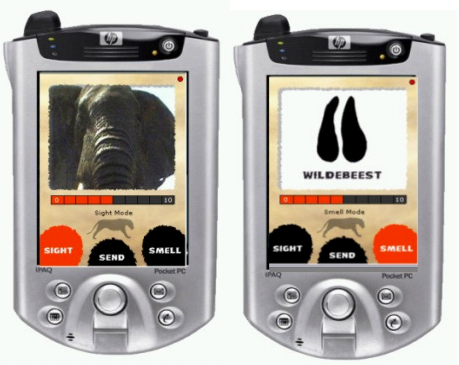
\includegraphics[scale=0.6]{fig/savannah}
	\caption{In Savannah \cite{Benford_Rowland_Hull_Reid_Morrison_Facer_Clayton_2004} users explore a virtual savannah through a smartphone}
	\label{fig:savannah}
\end{figure}
\\
\noindent Pirates is another game for mobile phones that - like Savannah - uses the location of players to provide different possibilities in the game \cite{Falk:2001:PPI:634067.634140}. Instead of using absolute location and using it to determine a location in the game in Pirates! the proximity between players is used. In Pirates!, the setting is an archipelago, and, like in Savannah, players are given different missions to accomplish. The game field is fitted with radio frequency proximity sensors and so are the mobile devices that players use to play the game. This allows for the sensing of what is referred to as \emph{player to place proximity} and \emph{player to player proximity} respectively. These different proximities are then used to provide different possibilities for the players in the game.
\\\\
Finally, Ardito et. al. present a mobile location-enhanced system that supports history learning for young students \cite{4351331}. The system supports the exploration of archeological sites by providing extra information through a mobile device. Moving around the archeological site, users are given small missions to accomplish. The users can identify a place described by the mission and either digit a place code or scan the place's visual tag to tell the system that the place has been identified. Having completed the last mission, the users are presented with a 3D representation of places they have explored. Fig. \ref{fig:ardito} shows the 3D representation of a furnace as presented to the users.

\begin{figure}
	\centering
	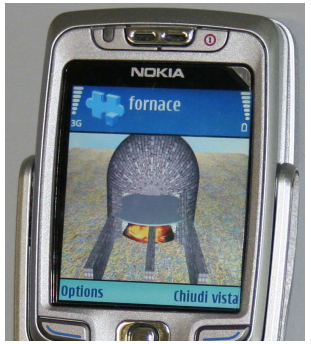
\includegraphics[scale=0.6]{fig/ardito}
	\caption{Ardito et. als \cite{4351331} system support history learning for young students through mobile interaction}
	\label{fig:ardito}
\end{figure}

\\\\
\noindent Several location-based applications are available for download from the digital marketplaces, and some have experienced great success already. foursquare is one of the most popular location based application. It's a social platform where users share their locations by 'checking in'. These check ins generate points and badges, allowing users to compete against each other in a race to get the most points. The competitive gaming aspects is further enhanced by the possibility to become Mayor of a given location - a title awarded the person who checks in the most. Gowalla\footnate{\url{http://gowalla.com}} was a social location based app that was sold to Facebook in 2012. Similar to foursquare\footnote{\url{http://foursquare.com/}} it allowed users to check in at different locations to receive awards. Users were awarded items which could be used in turn to create new places. The app also awarded users \emph{pins} for complete trips; checkins at a series of specified locations. WHERE\footnote{\url{http://where.com/}} is a location-based app allowing users to share information location specific information. The types of information can be ratings of places, discounts in stores or the price of gas at a gas station. WHERE makes this kind of user-generated information easily available to users in the vicinity. WHERE also has a strong business model where companies can use WHERE to promote themselves. 
% subsection agumented_spaces (end)

\subsection{End user programming} % (fold)
\label{sub:end_user_programming}
The creation of location-enhanced applications have become easier with the introduction of location-sensing mobile devices and programming API's that support obtaining location data. Now, the location sensors and the access to their information is directly embedded in to the environment in which location applications will run. While creating location based apps still requires programming experience, some methods have been proposed to abstract the creation of location based apps to move it from a programming to an end-user programming context. 
\\\\
Topiary is a tool for prototyping location-enhanced applications \cite{Li:2004:TTP:1029632.1029671}. It is meant for designers who want to prototype and test new location-enhanced applications. The Topiary tool is split in to three workspaces; Active Map, Storyboard, and Test. The Active Map is used to model the entities in the system. The user can upload a map and draw areas of interest while adding people and things of interest as seen in fig \ref{fig:topiary}.

\begin{figure}
	\centering
	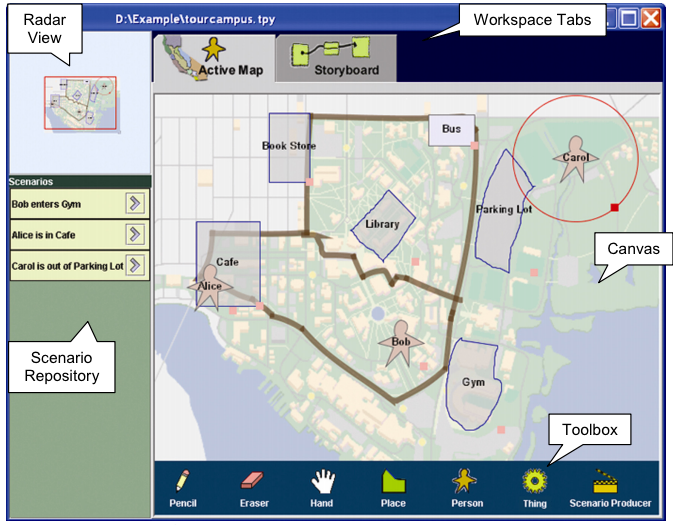
\includegraphics[scale=0.4]{fig/topiary}
	\caption{In Topiary \cite{Li:2004:TTP:1029632.1029671} users can annotate a map with people, places and things to create location-enhanced scenarios}
	\label{fig:topiary}
\end{figure}
\\
\noindent Using these places, persons and things, users can model contextual scenarios. In the Storyboard workspace, the scenarios sketched can then be used to create conditions and links. Finally, the prototype can be run on a mobile device using the Test workspace. While Topiary can be used to create location-based prototypes it only supports obtaining location through PlaceLab (wifi positioning) - more fine-grained location information will have to be provided through a wizard updating the locations of the tracked users. 
\\\\
Dey et. al. present a CAPpella, a tool enabling end-users to create context-aware behavior \cite{Dey:2004:CPD:985692.985697}. Rather than enabling users to create context-aware applications, a CAPpella enables users to model context-aware behavior. Users can hook up sensors with a CAPpalla and record the sensor data. Afterwards this data can be annotated with information telling the program that a specific event has occurred - e.g. a user can mark a period of time where the sound level is high. Repeating this step will train the system to automatically recognize events in the sensor data - e.g. when the sound is loud. These events can then trigger user-defined actions like turning the light on. While location information is not regarded in this system, it is easy to see how location sensors could be supported. Fig. \ref{acappella} shows the a CAPpella UI while being trained to turn on the lights when for a meeting.

\begin{figure}
	\centering
	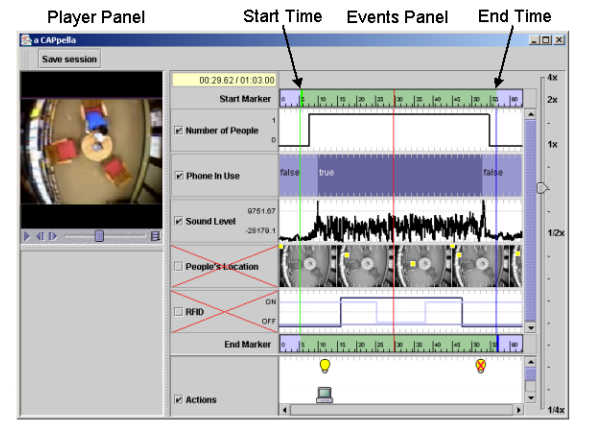
\includegraphics[scale=0.4]{fig/acappella}
	\caption{Training a CAPpella \cite{Dey:2004:CPD:985692.985697} to turn on and off the lights in different situations}
	\label{fig:acappella}
\end{figure}
\\\\
\noindent Häkkilä et. al. present Context Studio \cite{springerlink:10.1007/11555261_73} - an application for mobile phones that allow users to model context aware behavior. Context Studio offers a number of predefined triggers and actions - all related to the functionality of the phone. Users can model context-aware behavior by adding rules to the phone. A rule specifies a number of triggers - preconditions that must be met - and an action to take when the conditions have been met. The triggers can be explicit user input such as buttons pressed or touch gestures performed or implicit sensed data such as sound-level or location. The actions are existing actions that the phone supports such as sending text messages, taking picture or switching to silent mode.
\\\\ 
With explosion of smart phones, businesses have also realized the potential of having an application to promote its products or services. This, in turn, have created a market for app-creation systems, where non-programmers can create simple smart phone applications. Of particular interest of our project is shoutem\footnote{\url{http://www.shoutem.com/}}. shoutem is a web based system for creating smart phone apps. Users can access a webpage to create, edit, and publish iOS\footnote{\url{http://www.apple.com/ios/}} and Android\footnote{\url{http://www.android.com/}} applications. shoutem incorporates location-based features by using foursquare. Users can add places to the app, and allow check-ins, events (like a party - not programming language events), and user uploaded location-specific comments, media etc. 
% subsection end_user_programming (end)
% section related_work (end)
